\subsection{Embedding: Complemented Type System Lattice}

{  \setbeamercolor{background canvas}{bg=sectioncolor}
\begin{frame}{\Challenge{3} Type Lattice}

  How to support types like \textcolor{greeny}{$Int\cap\overline{Number}$} in Scala?

  \begin{itemize}
  \item Support \Emph{complemented type lattice}
  \item Embed a dynamic type system into an existing programming language.
  \item Answer type membership and subtype questions.
  \end{itemize}

\end{frame}
}



\newsavebox\tdast
\begin{lrbox}{\tdast}
  \begin{minipage}{11cm}
    %% dont re-indent this file
\begin{lstlisting}[style=scalaioScala]
val Int:SimpleTypeD      = SAtomic(classOf[Int])
val Double:SimpleTypeD = SAtomic(classOf[Double])

val td:SimpleTypeD = SOr(Double, SAnd(Int, SNot(SEql("X"))))
\end{lstlisting}

  \end{minipage}
\end{lrbox}


\begin{frame}{Example \code{SimpleTypeD} Expression Tree: AST}
  \usebox\tdast

  \medskip

  \centering

  \scalebox{0.7}{% Modeled after the following
% A simple Tree
% Author: Stefan Kottwitz
% https://www.packtpub.com/hardware-and-creative/latex-cookbook
\documentclass[border=10pt]{standalone}
\usepackage{tikz}
\begin{document}
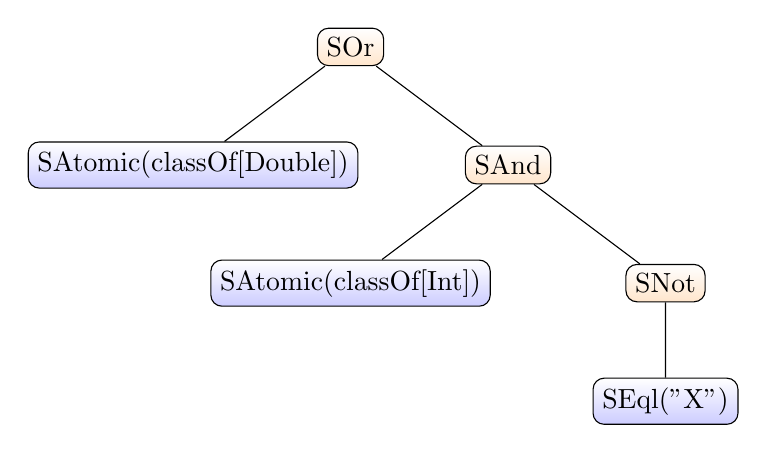
\begin{tikzpicture}[sibling distance=10em,
  every node/.style = {shape=rectangle, rounded corners,
    draw, align=center,
    top color=white, bottom color=orange!20}]]
    \tikzstyle{level 1}=[sibling distance=40mm]
    \tikzstyle{level 2}=[sibling distance=40mm]
    \tikzstyle{level 3}=[sibling distance=40mm]
  \node {SOr}
    child { node [bottom color=blue!20] {SAtomic(classOf[Double])} }
    child { node {SAnd}
      child { node [bottom color=blue!20] {SAtomic(classOf[Int])} }
      child { node {SNot} 
        child { node [bottom color=blue!20] {SEql("X")} } } } ;
\end{tikzpicture}
\end{document}
}
  \begin{itemize}
  \item A type designator is an expression tree (AST).
  \item Leaf nodes interface to Scala classes via \code{SAtomic(...)}. 
  \item \ldots and to literal Scala values via \code{SEql(...)}
  \item \ldots and to predicate functions via \code{SSatisfies(...)}
 \end{itemize}
\end{frame}


\begin{frame}{\code{SimpleTypeD} class quasi-ADT}
  \scalebox{0.95}{% Modeled after the following
% A simple Tree
% Author: Stefan Kottwitz
% https://www.packtpub.com/hardware-and-creative/latex-cookbook
\documentclass[border=10pt]{standalone}
\usepackage{tikz}
\begin{document}
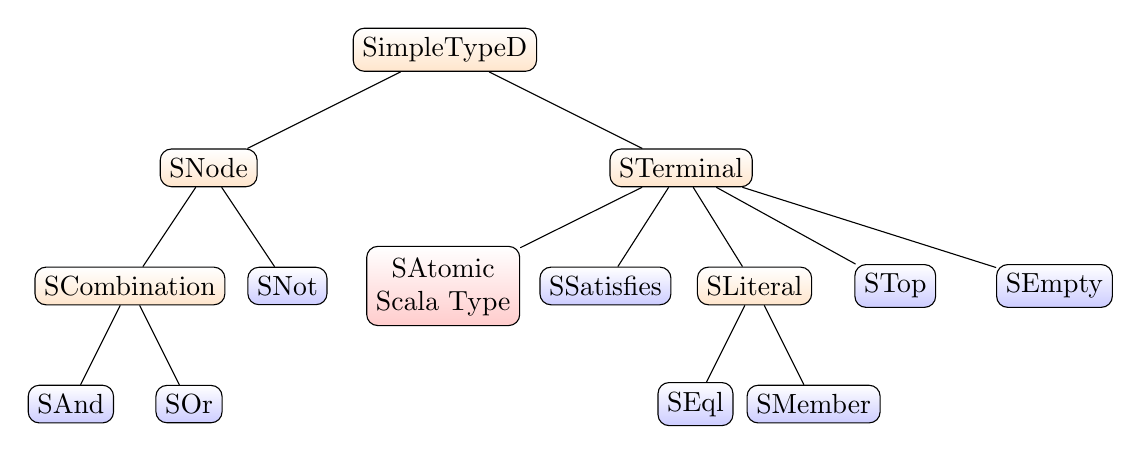
\begin{tikzpicture}[sibling distance=10em,
  every node/.style = {shape=rectangle, rounded corners,
    draw, align=center,
    top color=white, bottom color=blue!20}]]
    \tikzstyle{level 1}=[sibling distance=60mm]
    \tikzstyle{level 2}=[sibling distance=20mm]
    \tikzstyle{level 3}=[sibling distance=15mm]
  \node [bottom color=orange!20] {SimpleTypeD}
    child { node [bottom color=orange!20] {SNode}
      child { node [bottom color=orange!20] {SCombination} 
        child { node {SAnd} }
        child { node {SOr} } }
      child { node {SNot} } }
    child { node [bottom color=orange!20] {STerminal}
      child { node [text height=20pt, right=0mm, top color=white, bottom color=red!20] {SAtomic\\Scala Type } }
      child { node [right=2mm] {SSatisfies} }
      child { node [right=2mm] [bottom color=orange!20] {SLiteral}
        child { node {SEql} }
        child { node {SMember} } }
      child { node [right=2mm] {STop} }
      child { node [right=0mm] {SEmpty} } } ;
\end{tikzpicture}
\end{document}
}

\end{frame}


%% \begin{frame}{Types}{What are Types?}
%%   \begin{itemize}
%%   \item Types as Sets
%%   \item Static
%%   \item Dynamic
%%   \end{itemize}
%% \end{frame}


%% \begin{frame}{SETS}{Simple Embedded Type System}

%%   \scalebox{1.0}{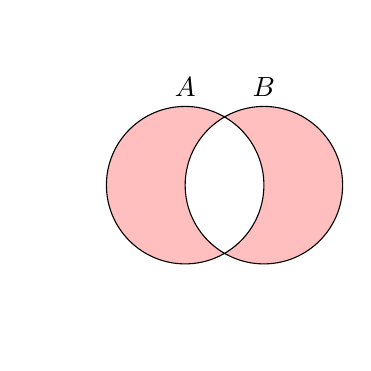
\begin{tikzpicture}[fill=pink]
% left hand
\scope
\clip (-2,-2) rectangle (2,2)
      (1,0) circle (1);
\fill (0,0) circle (1);
\endscope
% right hand
\scope
\clip (-2,-2) rectangle (2,2)
      (0,0) circle (1);
\fill (1,0) circle (1);
\endscope
% outline
\draw (0,0) circle (1) (0,1)  node [text=black,above] {$A$}
      (1,0) circle (1) (1,1)  node [text=black,above] {$B$};
\end{tikzpicture}
}

%%   \begin{itemize}
%%   \item   Extends type system of language (Scala, Python, Clojure)
%%   \item   Supports intersection, union, complement.
%%   \item   Supports \Emph{Boolean membership check}.
%%   \item   Supports \Emph{semi-Boolean subtype check}.
%%   \end{itemize}
%% \end{frame}


%% \begin{frame}{SETS}{Lattice}
%%   \begin{columns}
%%     \begin{column}{0.35\textwidth}
%%         %% By Watchduck author "T. Piesk", "Tilman Piesk" or
%%       %% "Watchduck". - Own work, CC BY 3.0,
%%       %% https://commons.wikimedia.org/w/index.php?curid=11155125
%%       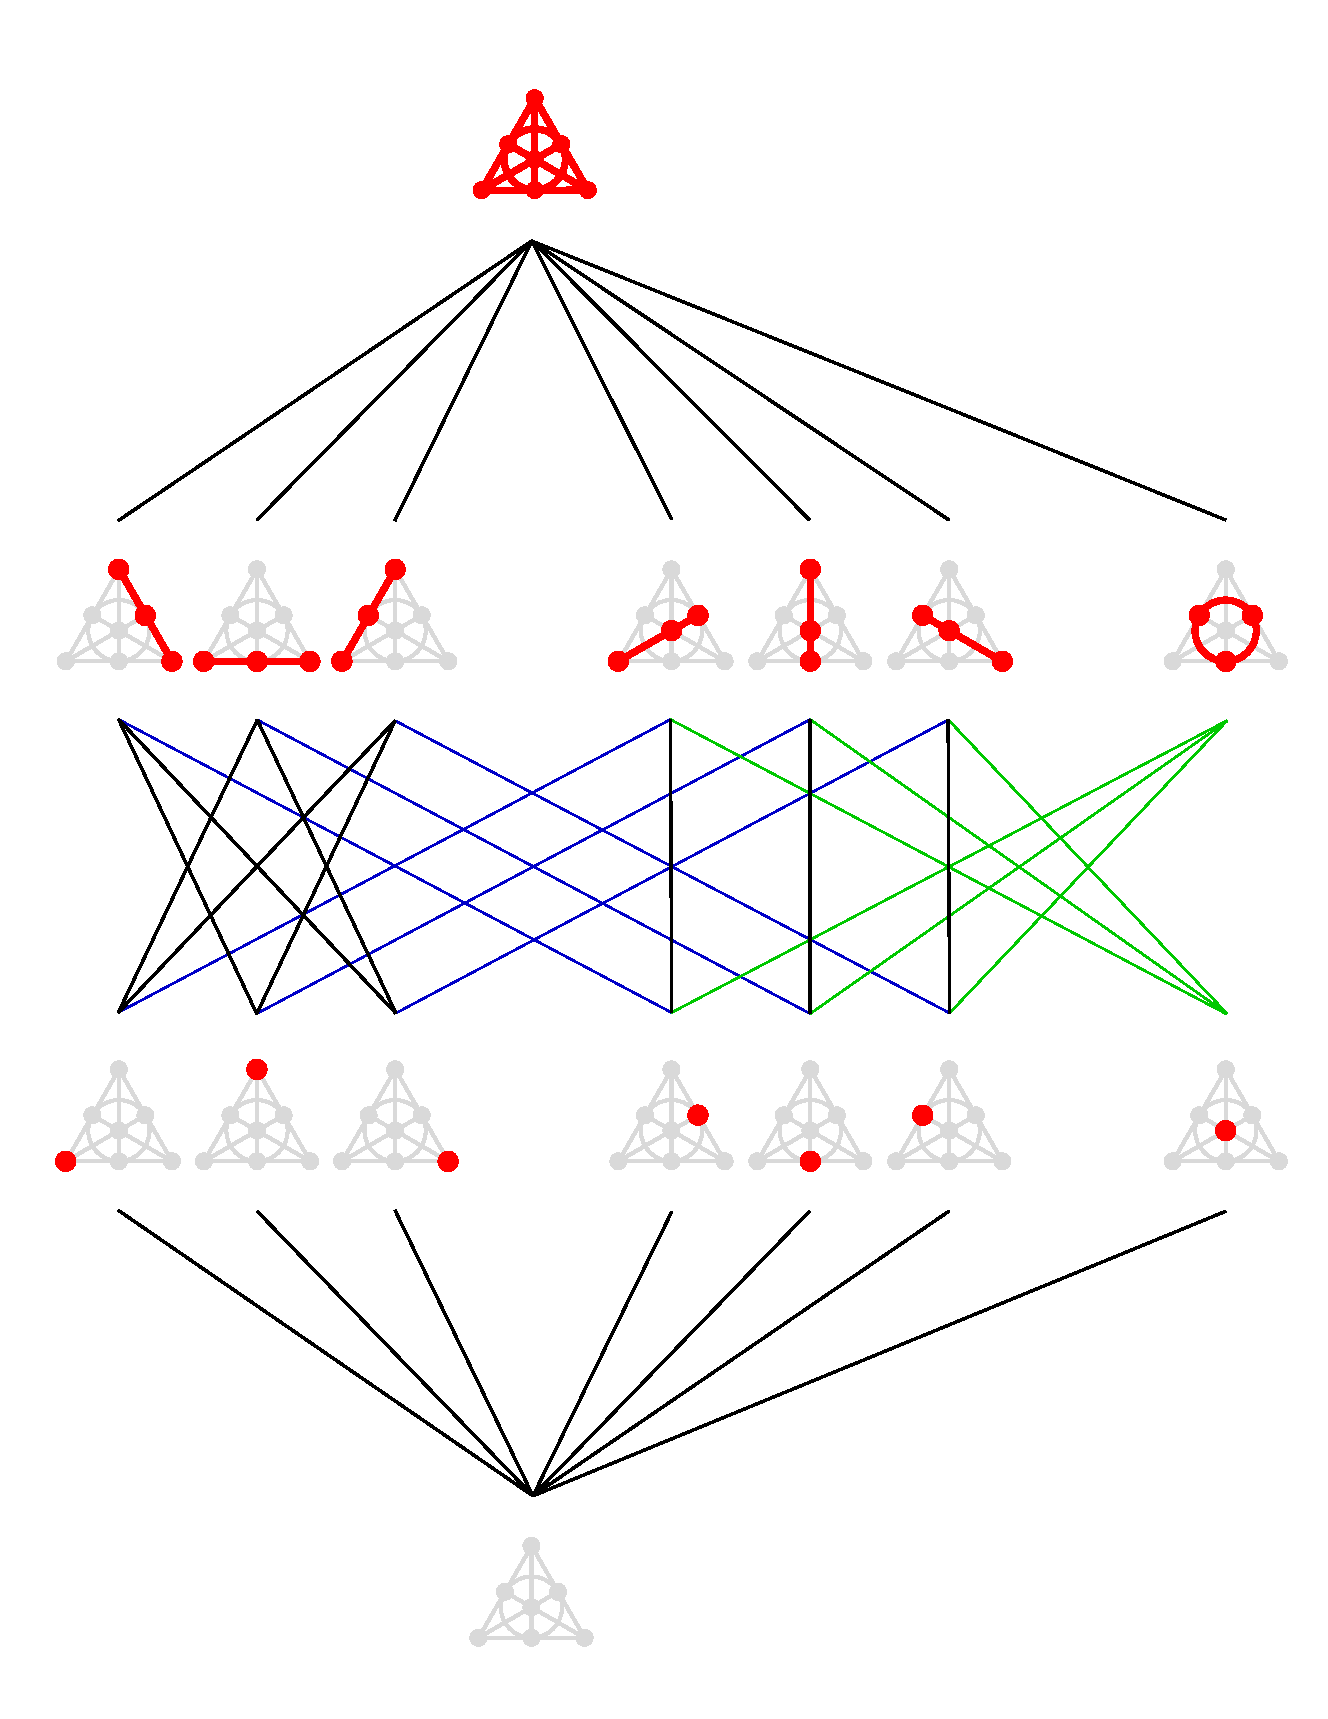
\includegraphics[height=6cm]{Fano_plane_Hasse_diagram} 
%%     \end{column}
%%     \begin{column}{0.65\textwidth}%%
%%       \Emph{Complemented lattice} of types.

%%       \medskip
      
%%   \begin{itemize}
%%   \item \code{SEmpty} and \code{STop}, empty and universal type
%%   \item \code{SAnd} and \code{SOr}, union and intersection
%%   \item \code{SNot} complement
%%   \end{itemize}      
%%     \end{column}
%%   \end{columns}
  
%%   \eg: \code{SOr(String, SAnd(Number,SNot(Int))) = String | (Number \& !Int)}


%% \end{frame}

%% \newsavebox\adtbox
%% \begin{lrbox}{\adtbox}
%%   \begin{minipage}{11cm}
%%     
\begin{lstlisting}[style=scalaioScala]
abstact class SimpleTypeD {...}
case class SNot(s: SimpleTypeD) extends SimpleTypeD {...}
case class SOr(override val tds: SimpleTypeD*) extends SimpleTypeD {...}
case class SAnd(override val tds: SimpleTypeD*) extends SimpleTypeD {...}
case class SAtomic(ct: Class[_]) extends SimpleTypeD {...}
object SEmpty extends SimpleTypeD {...}
object STop extends SimpleTypeD {...}
case class SSatisfies(f: Any => Boolean, printable:String) extends SimpleTypeD {...}
\end{lstlisting}

%%   \end{minipage}
%% \end{lrbox}






%% \begin{frame}{SimpleTypeD}{Interface to built-in type system}
  
%%   \begin{itemize}
%%   \item \code{SAtomic} encapsulates built-in type \code{Class[\_]}\\
%%     \eg, \code{SAtomic(classOf[Int])}.
%%   \item \code{SMember} and \code{SEql}, explicit types, encapsulates designated values\\
%%     \eg, \code{SEql("hello")}, \code{SMember(1,2,3)}
%%   \item \code{SSatisfies} encapsulates any predicate: \code{Any => Boolean}\\
%%     \eg, \code{SSatisfies(primep)}.
%%   \end{itemize}
%% \end{frame}


\newsavebox\membershipbox
\begin{lrbox}{\membershipbox}
  \begin{minipage}{11cm}
    %% dont re-indent this file
\begin{lstlisting}[style=scalaioScala]
SAtomic(classOf[Int]).typep(-42) // returns true

// returns true
(SAtomic(classOf[String]) || SAtomic(classOf[Int])).typep(7)


// define predicate
def oddp(a:Any):Boolean = {
  a match
    case a:Int => a % 2 != 0
    case _ => false
}

SSatisfies(oddp).typep(36)  // returns false
\end{lstlisting}

  \end{minipage}
\end{lrbox}

\begin{frame}{Type Membership Predicate}
  \emph{Boolean} type membership question is \Emph{always answerable}.

  \usebox\membershipbox
\end{frame}

\newsavebox\subtypebox
\begin{lrbox}{\subtypebox}
  \begin{minipage}{11cm}
%% dont re-indent this file
\begin{lstlisting}[style=scalaioScala]
val Str:SimpleTypeD = SAtomic(classOf[String])
val Int:SimpleTypeD = SAtomic(classOf[Int])
val Num:SimpleTypeD = SAtomic(classOf[Number])

Str.subtypep(Int)  // returns Some(false)
Int.subtypep(Num)  // returns Some(true)
SSatisfies(oddp).subtypep(Int) // returns None
\end{lstlisting}

  \end{minipage}
\end{lrbox}



\begin{frame}{Subtype Predicate}

  \emph{Semi-Boolean} Subtype predicate \Emph{sometimes unanswerable}.

  \usebox\subtypebox

  Unanswerable because:
  \begin{itemize}
  \item Impossible to compute, \eg \code{SSatisfies}.
  \item Code is incomplete.
  \item JVM supports run-time loaded classes.
  \item Limitations of support libraries (discussed later).
  \end{itemize}

\end{frame}

\begin{frame}{Simple Embedded Type System: SETS}

  At the point, \Emph{what have we done}?

  \begin{itemize}
  \item Wrapped the Scala type system
  \item ... with a simple type system
  \item ... which supports a complemented type lattice
  \item ... with membership Boolean predicate
  \item ... with subtype semi-Boolean predicate
  \item ... which supports reflection
  \end{itemize}

  \medskip

  Cf: \textit{A Portable, Simple, Embeddable Type System} [Newton, Pommellet] 2021 ELS

\end{frame}
